\title{BT5110 Data Management and Warehousing}

\subtitle{Tutorial 3: Aggregate and Nested Queries}

\author{Mark Meng Huasong}

\institute[National University of Singapore] % (optional, but mostly needed)
{
	School of Computing\\
	National University of Singapore
}

\titlegraphic{
	
\includegraphics[width=2cm]{nus-logo}
}

\date{6 - 10 Sep, 2021}

\begin{frame}
	\titlepage
	\begin{tcolorbox}
		\begin{center}
			{\scriptsize \textcolor{red}{All the materials within presentation slides are protected by copyrights.\\
					It is forbidden by NUS to upload these materials to the Internet.}}
		\end{center}
	\end{tcolorbox}
\end{frame}

\begin{frame}[fragile]{Quick Recap: End of Last Tutorial}
	What we have done in the last week:\\\vspace{5pt}
	(1) Write simple a query with arithmetic, comparison \& logical operators;\\
	(2) Write a table joining query (CROSS JOIN and INNER JOIN);\\
	(4) Write simple a query with the set operators.\\\vspace{5pt}
	
	Summary of our database (\# of rows):\\\vspace{5pt}
	\centering
	\begin{tabular}{|c|c|c|c|c|} \hline
		\textbf{book} & \textbf{student} & \textbf{copy} & \textbf{loan} & \textbf{department}\\ \hline
		311 & 105 & 1244 & 4976 & 13 \\ \hline
	\end{tabular}
	
	\begin{figure}
		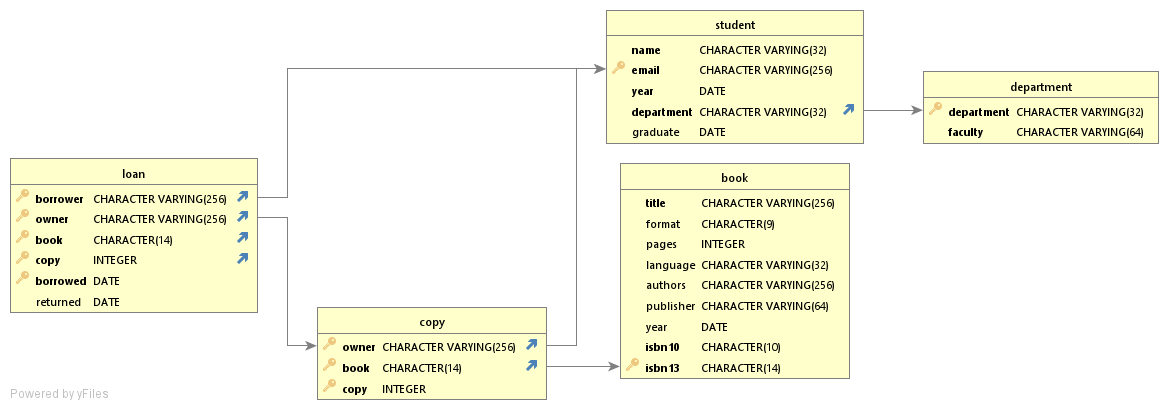
\includegraphics[width=1\textwidth]{t1/images/t1-end.png}
	\end{figure}\vspace{-10pt}
	{\tiny(plotted by DbVisualizer)}
\end{frame}

\section*{Question 1 Aggregate Queries}

\begin{frame}[fragile]{Question 1 (a)}
\underline{How many} loans involve an owner \underline{and} a borrower from the same department?\\ \vspace{10pt}

\textbf{Solution:}\\
\begin{lstlisting}
SELECT COUNT(*)
FROM loan l, student s1, student s2
WHERE l.owner = s1.email 
AND l.borrower = s2.email
AND s1.department = s2.department;
\end{lstlisting}
\vspace{10pt}
You should have \textcolor{red}{\textbf{502}} observed in the output. 
\end{frame}


\begin{frame}[fragile]{Question 1 (b)}
For \underline{each} faculty, print the \underline{number of loans} that involve an owner \underline{and} a borrower from this faculty?
\vspace{10pt}

\textbf{Solution:}\\
\begin{lstlisting}
SELECT d1.faculty, COUNT(*)
FROM loan l, student s1, student s2, department d1, department d2
WHERE l.owner = s1.email 
	AND l.borrower = s2.email
	AND s1.department = d1.department
	AND s2.department = d2.department
	AND d1.faculty = d2.faculty
GROUP by d1.faculty;
\end{lstlisting} \vspace{10pt}
\end{frame}

\begin{frame}[fragile]{Question 1 (b) Cont.}

The output should be like as follows (for your reference).\\ \vspace{10pt}
\begin{lstlisting}[style=terminial]
             faculty               | count
-----------------------------------+-------
Faculty of Arts and Social Science |   379
Faculty of Engineering             |    82
Faculty of Science                 |   239
School of Computing                |   529
(4 rows)	
\end{lstlisting}
\end{frame}


\begin{frame}[fragile]{Question 1 (c)}
What are the \underline{average} and the \underline{standard deviation} of the \underline{duration} of a loan? \textcolor{brown}{(assume today is 2010-12-31)}\\ \vspace{10pt}

Recap of Q1 (d) of Tutorial 2: print the duration of each loan:
\begin{lstlisting}
SELECT l.book, ((CASE WHEN l.returned ISNULL 
	THEN '2010-12-31'
	ELSE l.returned END) - l.borrowed + 1) AS duration 
FROM loan l
ORDER BY l.book ASC, l.duration ASC;
\end{lstlisting}

\textcolor{red}{How can we reuse this code?}
\end{frame}


\begin{frame}[fragile]{Question 1 (c) Cont.}
	
\textbf{Solution:}

\begin{lstlisting}
SELECT AVG((CASE WHEN l.returned ISNULL 
		THEN '2010-12-31'
		ELSE l.returned END) - borrowed + 1),
	STDDEV_POP((CASE WHEN l.returned ISNULL 
		THEN '2010-12-31'
		ELSE l.returned END) - borrowed + 1)
FROM loan l;
\end{lstlisting}
\vspace{5pt}
The output should be as follows.
\begin{lstlisting}[style=terminial]	
         avg         |     stddev_pop
---------------------+---------------------
 41.4963826366559486 | 38.4206806387009364
(1 row)	
\end{lstlisting}
\vspace{5pt}
\textbf{Extra}: \textcolor{brown}{Can we use nested query to simplify it?}
\end{frame}


\begin{frame}[fragile]{Question 1 (c) Cont.}
	
\textbf{Solution (nested version):}
\begin{lstlisting}
SELECT AVG(temp.duration), STDDEV_POP(temp.duration)
FROM (SELECT ((CASE
		WHEN l.returned ISNULL 
		THEN '2010-12-31'
		ELSE l.returned END) - l.borrowed + 1) AS duration 
	FROM loan l) AS temp;
\end{lstlisting}
\end{frame}

\section*{Question 2 Nested Queries}

\begin{frame}[fragile]{Question 2 (a)}
Print the titles of different books that have \underline{never been borrowed}. Use a nested query.\\ \vspace{5pt}

\textcolor{brown}{Which tables are involved in this nested query?}
\begin{figure}
	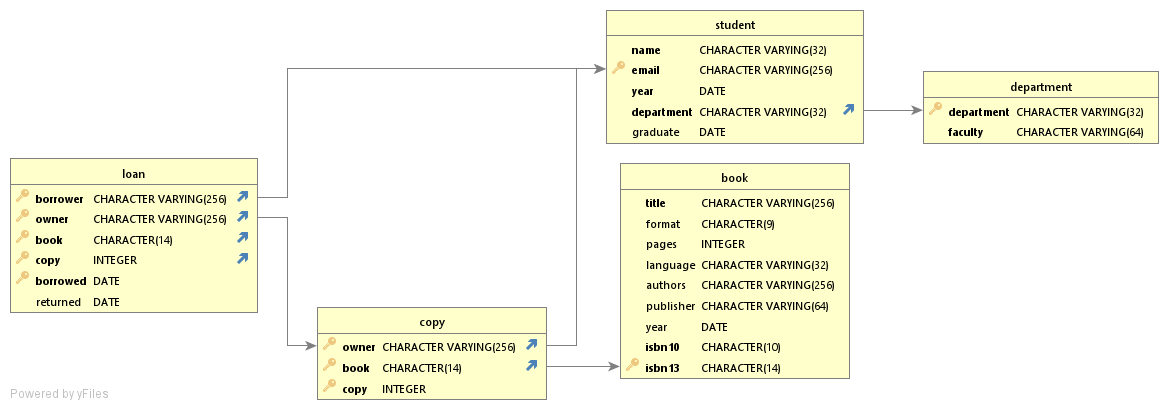
\includegraphics[width=1\textwidth]{t1/images/t1-end.png}
\end{figure}\vspace{-10pt}
{\tiny(plotted by DbVisualizer)}
\end{frame}

\begin{frame}[fragile]{Question 2 (a) Cont.}
\textbf{Solution}:

\begin{lstlisting}
SELECT b.title 
FROM book b
WHERE b.ISBN13 NOT IN (
	SELECT  l.book 
	FROM loan l);
\end{lstlisting}\vspace{5pt}

...or, equivalently,

\begin{lstlisting}
SELECT b.title 
FROM book b
WHERE b.ISBN13 <> ALL (
	SELECT l.book 
	FROM loan l);
\end{lstlisting}\vspace{5pt}

You should observe \textcolor{red}{\textbf{no}} record given in the output. 
\end{frame}

\begin{frame}[fragile]{Question 2 (b)}
Print the name of the different students who \underline{own} a copy of a book that they have \underline{never lent} to anybody.\\ \vspace{5pt}

\textcolor{brown}{Which tables are involved in this nested query?}
\begin{figure}
	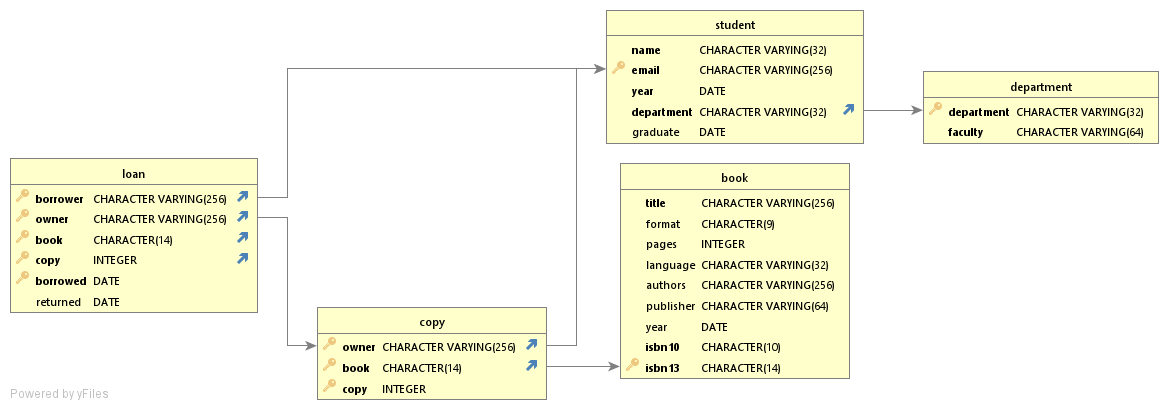
\includegraphics[width=1\textwidth]{t1/images/t1-end.png}
\end{figure}\vspace{-10pt}
{\tiny(plotted by DbVisualizer)}
\end{frame}

\begin{frame}[fragile]{Question 2 (b) Cont.}
\textbf{Solution}:
	
\begin{lstlisting}
SELECT s.name 
FROM student s
WHERE s.email IN 
	(SELECT c.owner
	FROM copy c
	WHERE NOT EXISTS (
		SELECT * 
		FROM loan l
		WHERE l.owner = c.owner
			AND l.book = c.book
			AND l.copy = c.copy));
\end{lstlisting}\vspace{5pt}
\end{frame}

\begin{frame}[fragile]{Question 2 (b) Cont.}
	
...or, equivalently,
	
\begin{lstlisting}
SELECT s.name 
FROM student s
WHERE s.email = ANY (
	SELECT c.owner
	FROM copy c
	WHERE NOT EXISTS (
		SELECT * 
		FROM loan l
		WHERE l.owner = c.owner
			AND l.book = c.book
			AND l.copy = c.copy));
\end{lstlisting}\vspace{5pt}
	
You should observe \textcolor{red}{\textbf{no}} record given in the output. \\

\begin{block}{Notice}
We can always use ``\texttt{<> ALL}'' as an equivalence of ``\texttt{NOT IN}''. Similarly, we can use ``\texttt{= ANY}'' as an equivalence of ``\texttt{IN}''
\end{block}	
\end{frame}

\begin{frame}[fragile]{Question 2 (c)}
For each department, print the names of the students who lent the \underline{most}.
\end{frame}


\begin{frame}[fragile]{Question 2 (c) Cont.}
\textbf{Solution}:
	
\begin{lstlisting}
SELECT  s.department, s.name, count(*)
FROM student s, loan l
WHERE l.owner = s.email
GROUP BY s.department, s.email
HAVING count(*) >= ALL
	(SELECT  count(*) 
	FROM student s1, loan l1
	WHERE l1.owner = s1.email
	AND s.department = s1.department
	GROUP BY s1.email);
\end{lstlisting}\vspace{5pt}
\end{frame}



\begin{frame}[fragile]{Question 2 (c) Cont.}
You should observe the output as follows.\\
\begin{lstlisting}[style=terminial-tiny]	
department |     name      | count
-----------+---------------+-------
Geography  | SEAH TECK KEE |    64
Geography  | ZHANG YUZHAO  |    64
EE         | WANG NA       |    60
CE         | TAY YONG MING |    68
Math       | HUANG WENXIN  |    76
CS         | LIU ZHENCAI   |    76
Geography  | DAVID HALL    |    64
ME         | GE DUO        |    64
Language   | NEELAM DEOL   |    68
Biology    | PENG JIAYUAN  |    80
IS         | ZHANG HONG    |    88
History    | ZENG YIHUI    |    60
Economics  | LI YUZHAO     |    60
Physics    | NI HANRAN     |    60
Chemistry  | XIE XIN       |    56
(15 rows)
\end{lstlisting}\vspace{5pt}
\begin{alertblock}{Warning}
	Notice that there are three such students in the department of \textbf{Geography}  (that is why one should almost never use TOP N queries). 	
\end{alertblock}
\end{frame}

\begin{frame}[fragile]{Question 2 (c) Cont.}
	
	
\textbf{Extra:} What if I insert the query below before we execute the solution?
\begin{lstlisting}
INSERT INTO department VALUES('Business Analytics', 'School of Computing');
INSERT INTO student VALUES('MARK MENG', 'markmeng@biz.nus.edu.sg', '2010-01-01', 'Business Analytics', '2014-01-01');
\end{lstlisting}
We expect the output to be like:\\
\begin{lstlisting}[style=terminial-tiny]	
	department         |     name      | count
	-------------------+---------------+-------
	Geography          | SEAH TECK KEE |    64
	Geography          | ZHANG YUZHAO  |    64
	EE                 | WANG NA       |    60
	CE                 | TAY YONG MING |    68
	Math               | HUANG WENXIN  |    76
	CS                 | LIU ZHENCAI   |    76
	Geography          | DAVID HALL    |    64
	ME                 | GE DUO        |    64
	Language           | NEELAM DEOL   |    68
	Biology            | PENG JIAYUAN  |    80
	IS                 | ZHANG HONG    |    88
	History            | ZENG YIHUI    |    60
	Economics          | LI YUZHAO     |    60
	Physics            | NI HANRAN     |    60
	Chemistry          | XIE XIN       |    56
	Business Analytics | MARK MENG     |    0
	(16 rows)
\end{lstlisting}
	\textcolor{brown}{For you to think about it... (out of scope of this tutorial)}
\end{frame}

\begin{frame}[fragile]{Question 2 (d)}
Print the emails and the names of the different students who borrowed \underline{all} the books authored by Adam Smith.

\textcolor{brown}{Can we make use of negation with nested query?}
\end{frame}

\begin{frame}[fragile]{Question 2 (d) Cont.}
\textbf{Solution}:
\begin{lstlisting}
SELECT s.email, s.name
FROM student s
WHERE NOT EXISTS (
	SELECT * 
	FROM book b
	WHERE authors = 'Adam Smith' AND NOT EXISTS (
		SELECT * 
		FROM loan l
		WHERE l.book = b.isbn13 AND l.borrower = s.email));
\end{lstlisting}\vspace{5pt}
\begin{lstlisting}[style=terminial]	
          email          |    name
-------------------------+-------------
 yeojiahao1989@yahoo.com | YEO JIA HAO
 (1 row)	
\end{lstlisting}
\end{frame}

\begin{frame}[fragile]{Question 2 (d) Cont.}

\textbf{Extra}: Can you spot the difference between the 2 queries below:
\begin{columns}[t]
\column{0.49\textwidth}
	
\begin{lstlisting}
SELECT s.email, s.name
FROM student s
WHERE NOT EXISTS (
	SELECT * 
	FROM book b
	WHERE authors = 'Adam Smith' 
	AND NOT EXISTS (
		SELECT * 
		FROM loan l
		WHERE l.book = b.isbn13 
		AND l.borrower = s.email));
\end{lstlisting}
\begin{lstlisting}[style=terminial-tiny]	
          email          |    name
-------------------------+-------------
 yeojiahao1989@yahoo.com | YEO JIA HAO
 (1 row)	
\end{lstlisting}
\column{0.5\textwidth}
\begin{lstlisting}
SELECT s.email, s.name
FROM student s
WHERE NOT EXISTS (
	SELECT * 
	FROM loan l
	WHERE l.borrower = s.email
	AND NOT EXISTS (
		SELECT *
		FROM book b
		WHERE b.authors = 'Adam Smith'
		AND l.book = b.isbn13));
\end{lstlisting}

\begin{lstlisting}[style=terminial-tiny]
          email          |      name
-------------------------+----------------
 glee@msn.com            | GERALDINE LEE
 tcy@hotmail.com         | TANG CHEE YONG
 awong007@msn.com        | ADELINE WONG
 tikki@gmail.com         | TIKKI TAVI
 rikki@gmail.com         | RIKKI TAVI
 (5 rows)
\end{lstlisting}
\end{columns}
\end{frame}
\begin{frame}{}
\centering  
For any further question, please feel free to email me:\vspace{10pt}

huasong.meng@u.nus.edu \vspace{20pt}

\begin{tcolorbox}
	\begin{center}
		\textcolor{red}{Copyright 2021 Mark H. Meng. All rights reserved.}
	\end{center}
\end{tcolorbox}

\end{frame}